\section{Képfeldolgozó megoldások kihívás-válasz implementálására}
\subsection{Alapok}
A kihívás - válasz megoldások célja a felhasználó-hitelesítés és -azonosítás valósidejűségének ellenőrzése. E nélkül a természetes és virtuális személy összehasonlítása után (amennyiben a két képen található arc megfelelő valószínűséggel azonos emberhez tartozik )  az authentikációt elfogadottnak vesszük.
Gondoljunk bele ennek a megoldásnak a sebezhetőségeibe. A legegyszerűbb feltörése a rendszernek, ha az elektronikus személyi igazolvánnyal történő azonosítás után a kamera elé helyezzük az igazolványt, képpel kamerának nézve. A használt képfeldolgozó szoftver nagy valószínűséggel fel fogja ismerni a képet, és magas százalékos valószínűséget fog dobni az összetartozóságra. Ennek a verziónak a sebezhetőségén kívánunk javítani kihívás - válasz megoldás implementálásával.
\subsection{Kihívás - válasz protokollok}
A számítógépes biztonság világában a kihívás - válasz protokoll-család lényege, hogy az authentikációban részt vevő felek közül az egyik oldal egy kérdést (kihívást) intéz a másik félhez, amire a sikeres authentikációhoz helyes választ kell adni. A legegyszerűbb ilyen protokoll a felhasználónév - jelszó alapú azonosítás, ahol a kihívás a jelszó kérése, a válasz pedig a helyes jelszó.
\\Ebben az esetben a  kihívás - válasz sikeressége érdekében szükséges valamilyen titkos adat megléte (itt a jelszó). Más megközelítésű felhasználás lehet például annak eldöntése, hogy egy szolgáltatást használni kívánó kérésről eldöntsük, hogy ténylegesen egy valódi ember indította. Egy széles körben elterjedt felhasználás, amikor a felhasználó egy szöveg képét kapja meg eltorzítva úgy, hogy azt a karakterfelismerő programok is a lehető legnehezebben olvassák, de az ember számára ne okozzon túl nagy nehézséget a karakterek felismerése. Ilyenkor semmi titkos adat megléte nem szükséges a sikeres használathoz.
\subsection{Első gondolatok}
Ennek a szakdolgozatnak célja nem különböző képfeldolgozó eszközök létrehozása, ami alapján ezeket a kihívásokat értékelni tudjuk. Leginkább publikusan elérhető third party lehetőségeket felkutatása volt a cél, amelyek önállóan tudnak feldolgozni képet vagy videót, majd bizonyos felismert tulajdonságokkal visszatérni a rendszerhez. Ezután ezeket a válaszokat feldolgozva eldönthető, hogy a bejelentkezést engedjük vagy megtagadjuk.
Alapvetően két típust különböztetünk meg elérhetőség szempontjából
\begin{itemize}
\item online
\item offline
\end{itemize}
Egy másik fajta osztályozás pedig működés szempontjából lehetséges
\begin{itemize}
\item implementálja a kihívás - válasz protokollt, így video-streamből egy igen/nem választ, esetleg egy százalékos valószínűséget ad
\item képfeldolgozó könyvtár / api, ami képet vár kérésben, válaszban pedig ennek valamilyen felismert tulajdonságaival tér vissza. Ezután nekünk kell eldönteni, hogy elfogadjuk-e az adott kihívásra érkezett választ
\end{itemize}

Az első komoly nehézség rögtön adja magát: amennyiben online megoldást választunk, az komoly adatforgalommal, és emiatt késleltetéssel járhat, pedig egy authentikációnál a gyorsaság nem elhanyagolható. Másik gyorsasági tényező az adott könyvtár/API képfeldolgozási sebessége különböző méretű/sebességű képek esetén. Ezt a feldolgozási időt drasztikusan csökkenteni lehet a képek méretének (és ezzel minőségének csökkentésével), de ez esetben komoly kérdés marad a képfeldolgozás minősége. Másik megoldás lehet a képek szürkeárnyalatossá alakítása, ezzel a képfeldolgozás sikeressége lehetséges, hogy kevésbé fog csökkenni mint egy sima tömörítésnél, de a méretet csökkentheti.
\\A képek mérete és ezzel a felhasznált sávszélesség, illetve sebesség két helyen számít. Először amikor a felhasználó eszköze (jelen esetben android okostelefon) rögzíti a videót, kiválaszt belőle valamennyi képkockát, majd továbbítja az azonosítást végző szervernek. Ezután pedig amikor ez a szerver továbbküldi egy third party alkalmazásnak. Jól látható, hogy a legkevesebb adatforgalommal az jár, ha már a felhasználó telefonján transzformációkat (tömörítés, szürkeárnyalatossá konvertálás) hajtunk végre. Ezzel a megközelítéssel a probléma viszont a felhasználói eszközök sokszínűsége: különböző erősségű telefonok különböző gyorsasággal tudják ezeket az alapvetően költséges műveleteket végrehajtani, szélsőséges esetben el is fogyhat a telefon alól a memória, ami az alkalmazás leállásához is vezethet.
\\Kézenfekvőnek látszódhat a költséges műveletek szerver oldalra való átcsoportosítása, hiszen ott a teljesítményt sokkal hatékonyabban tudjuk maximalizálni, monitorozni, végső esetben pedig több erőforrást adni. Ám ez esetben pedig egy erős minőségű kamerával készített pár másodperces videó komoly adatforgalommal járna, ami mobilnet esetében kifejezetten kerülendő.
Ezeket a kérdéseket mindenképp körül kell járni a tesztelés szakaszában, és a legoptimálisabbat megtalálni.
\\Összegezve  a fenti gondolatokat a következőket érdemes feljegyezni:

\begin{center}
	\begin{tabular}{|p{2cm}|p{3cm} |p{3cm} | p{3cm}|p{3cm}|}
   	\hline
	\textbf{Kép transzformációk helye} & \textbf{Sebesség} & \textbf{Adatforgalom} & \textbf{Képfeldolgozás minősége} &\textbf{ Hibalehetőségek} \\ \hline
	Nincs transzformáció & Adatforgalom sebessége & Legnagyobb & Legjobb & Kevés \\ \hline
	Felhasználó eszközén & Felhasználó eszközének minőségétől függ, plusz kétszeresen csökkentett adatforgalom sebessége & Legalacsonyabb & Képfeldolgozó szolgáltatás minőségétől függ & Ha gyenge a felhasználó eszköze, az alkalmazás nagyon lelassulhat, esetleg le is állhat \\ \hline
	Alkalmazás-szerveren & Egyszeresen csökkentett adatforgalom sebessége, plusz a szerver transzformációinak sebessége & Felhasználó szempontjából legnagyobb & Képfeldolgozó szolgáltatás minőségétől függ & Kevés\\ \hline
	\end{tabular}
\end{center}

A szakdolgozat keretein belül a második esetet, tehát a felhasználó eszközén történő transzformációt valósítottuk meg. A tesztelés feladata lesz a megfelelő paraméterek beállítása a képtömörítéshez, hogy minimalizáljuk azt az adatmennyiséget illetve sebességet, ami az adott képfeldolgozó eszköz megbízható működéséhez még szükséges.

\subsection{Képfeldolgozó eszközök}
Több online illetve offline képfeldolgozási lehetőséget vizsgáltunk meg, ezeknek egy része számunkra jelenleg nem használható, vagy használata nem fér bele a szakdolgozat kereteibe. A jelenlegi kihívás - válasz megoldásunk arc jobbra illetve balra fordulását keresi, illetve a két arc összetartozóságát állapítja meg, így elsősorban erre kihegyezve jegyeztük fel a talált lehetőségeket, de a jövőbeni fejlesztéseket szem előtt tartva más kihívás - válasz megoldásokra való használhatóságot is figyeltünk.
\subsubsection{Google Cloud Vision}
A Google Cloud Vision API \cite{GoogleCloudVision} A Google Cloud Platform Machine Learning moduljában található többek között a Cloud Speech API, és Cloud Translation API -val.
\\A számunkra érdekes Vision API egy képről az alábbi tulajdonságokat képes megállapítani:
\begin{itemize}
\item Különböző tárgyakat, élőlényeket, objektumokat ismer fel a képen és pozícionál
\item Tartalom moderálásra használható, szűrhet felnőtt, hamisított, erőszakos tartalomra vagy orvosi részleteket tartalmazó részekre (amik szintén rossz hatással lehetnek arra fel nem készült személyek számára)
\item Hasonló képeket keres az interneten, így például egy arcról eldöntheti, hogy melyik celebre hasonlít a legjobban
\item Visszaadja a felismert képeket minden tulajdonságukkal (szemöldök, száj pozíciók, stb.), illetve a felismert érzelmeket. Ezen felül megbízhatósági értékeket is küld válaszul, mégpedig "detectionConfidence" és "landmarkingConfidence" néven. Előző annak a a százalékos megbízhatósági értéke, hogy a felismert arc tényleg egy emberi arc, második esetben pedig a különböző arcon felismert elemek meghatárzosásának pontossága. Alacsony "landmarkingConfidence" esetén a fej elfordulás megbízhatatlan lehet, ezt kihasználhatjuk hibás eredmények felismerésében és elvetésében.
\end{itemize}

Az utolsó pontot tudjuk mi ez esetben kihasználni, mégpedig a visszaadott arc pozícióját, ami a Roll, Tilt, Pan hármasból a Pan (A szokásos fejelfordulás esetén használt megnevezés a "yaw", amit az API leírása szerint itt a Pan érték ad vissza).
\\Nagyon fontos a különböző API-k vizsgálatakor, hogy mekkora elfordulásig ismerik fel az arcokat a képen. Első tesztnek 2 képet használtam, egy picit elfordítottat és egy nagyon elfordítottat (ebben az esetben csak 1 szem látszódik).
Az eredmények (1. ábra, 2. ábra): \\

\begin{figure}[h]
 \begin{minipage}{.5\textwidth} 
\centering
    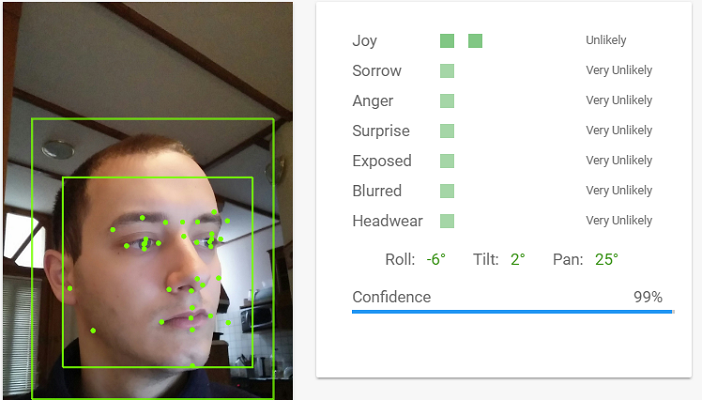
\includegraphics[scale=0.3]{img/cloud_vision_left}
    \caption{Balra néző kép, 25 fokos becsült elfordulás}
 \end{minipage}
 \begin{minipage}{.5\textwidth} 
\centering
     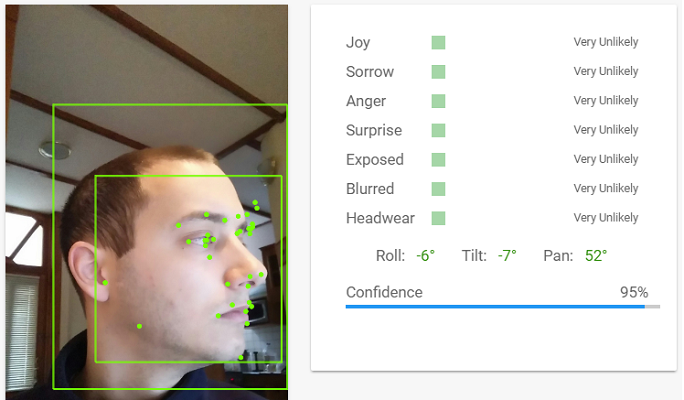
\includegraphics[scale=0.3]{img/cloud_vision_very_left}
     \caption{Balra néző kép, 52 fokos becsült elfordulás}
 \end{minipage}
\end{figure}

Vizsgáljuk meg külön mi történik a feldolgozás eredményével a komolyabb minőségromlás esetén. A feltöltendő képeket az eredeti ~500kb-ról ~40kb-ra csökkentettem, a minőségromlás szemmel látható. Hasonlítsuk össze az erre a két képre adott eredményt (3.ábra, 4.ábra)
\begin{figure}[h]
 \begin{minipage}{.5\textwidth} 
\centering
    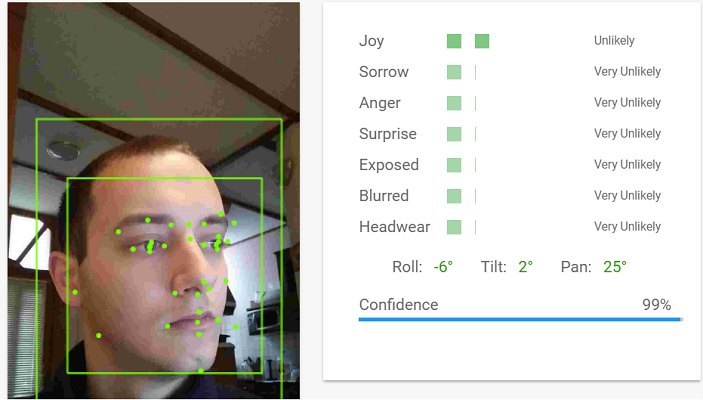
\includegraphics[scale=0.3]{img/cloud_vision_left_compressed}
    \caption{Balra néző tömörített kép, 25 fokos becsült elfordulás}
 \end{minipage}
 \begin{minipage}{.5\textwidth} 
\centering
     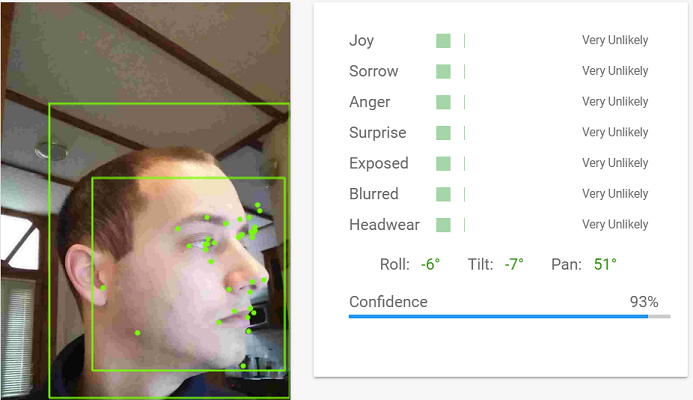
\includegraphics[scale=0.3]{img/cloud_vision_very_left_compressed}
     \caption{Balra néző tömörített kép, 51 fokos becsült elfordulás}
 \end{minipage}
\end{figure}

Jól látható, hogy jelentős méretcsökkentésre a feldolgozás megbízhatósága (a kék sávval jelzett "confidence" érték, ami a visszaadott "detectionConfidence" tulajdonság) 95\%-ról 93\%-ra változott abban az esetben, amikor a célszemély csak egyik szeme látszódik, a visszaadaott tulajdonságok pedig nagyvonalakban megegyeznek. 
Az eredmények láttán megállapítható, hogy a Google Cloud Vision széles skálán érzékeli az elfordulást, még akkor is, amikor a célszemély egyik szeme látszódik csak (ugyan ilyenkor az arc tulajdonságainak illesztése nem pontos, de az elfordulás mértéke hasonló), és tömörítésre sem érzékeny.
\\A probléma, hogy önmagában ez az API kevés lenne az elvárt működés implementálására, mivel arcösszehasonlítást nem tartalmaz. Így ha mégis a használat mellett döntünk, az összehasonlító modult egy másik eszközzel kell megoldani.

\subsubsection{IBM Watson}
Érdemes megvizsgálni, hogy az IBM Watson képfeldolgozó modulja (Visual Recognition \cite{IBMWatson}) mit tud adni nekünk a mi témakörünkben. 
\begin{itemize}
\item megbízhatósági pontszámmal csoportokba sorolja a képeket, ami csoportosításokra használható (pl.: Person, female, bridesmaid)
\item felismeri az arcokat, és visszaadja a pozíciókat, életkort tippel (minimum és maximum értékkel), illetve a felismert arc nemét állapítja meg.
\end{itemize}

A dokumentációban \cite{WATSON_DETECT} mélyebbre ásva sem lehet találni semmi olyan visszaadott értéket, ami az arcelforduláshoz segítséget adna, így megállapítható hogy nem lesz segítségünkre ez az API.

Arc összehasonlítás szempontból is érdemes lehet megvizsgálni a Collections BETA\cite{WATSON_COLLECTIONS} verzióban lévő API-ját. A működési mechanizmus nagyon hasonló más collections típusú arcösszehasonlítást tartalmazó szolgáltatásokhoz. Először hozzáadjuk a képet egy általunk választott gyűjteményhez, majd egy már feltöltött képhez hasonlóakat tudunk keresni egy adott gyűjteményben. Ez a megoldás akár segíthet is arcösszehasonlításban, de ez esetben minden regisztráció után a képet egy új gyűjteményben kéne elhelyezni, majd ebben a gyűjteményben keresni később, ám nem erre lett elsősorban létrehozva ez a szolgáltatás. Az alapötlet az, hogy metadata adatokat lehet csatolni a feltöltött képekhez (pl.: név), így például egy visszatérő felhasználót név szerint tudnánk már szólítani. Ráerőltethető valamilyen szinten az összehasonlítás is, de elsősorban olyan szolgáltatást kéne keresni, ami két képről dönti el hogy egyeznek-e, és a képeket se kelljen tárolni harmadik félnél. Ezek alapján az IBM Watson ezen megoldását elvethetjük.

\subsubsection{Google Mobile Vision}
A Google Mobile Vision\cite{GMV} egy offline, iOS illetve Android eszközökön futó arcfelismerő szolgáltatás. Óriási előny hogy offline, viszont hátrány hogy nem portolható át szerveroldalra, így önmagában nem használható a mi céljainkra. Érdemes ugyan megfontolni azt, hogy jelenlegi működés alapján egy több másodperc hosszú videóból kiválasztunk N darab képkockát, és azt továbbítjuk a szervernek. Ha pontosan tudnánk, hogy a felhasználó mikortól, meddig mozdította a fejét, akkor a felküldendő képkockák mennyiségét csökkenteni lehetne, illetve későbbi precízebb felismerést (pl.: pislogás felismeréséhez egy nagyon kicsi intervallumban sok kép szükséges a gesztikuláció gyorsaságából adódóan) is segíthetünk, ha tudjuk hogy a hosszabb intervallumban hol található pontosan a számunkra érdekes részlet.
\\Problémát okozhat viszont ebben az esetben a telefonok minősége, és így a feldolgozás gyorsasága. Meg kell találni azt a határt, ahol már nem érdemes előfeldolgozni a képeket, mert több időbe telne, mint feldolgozás nélkül küldeni válogatás nélkül.
\begin{figure}[h]
\centering
  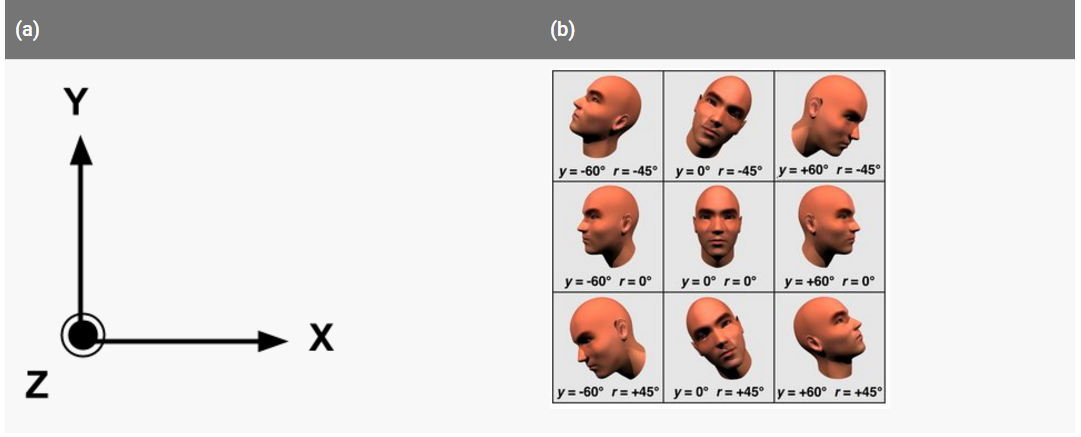
\includegraphics[scale=0.5]{img/gmv}
    \caption{A Google Moblie Vision által felismert elfordulási szögek (X tengely egyelőre inaktív)  \cite{GMV_ANGLES}}
\end{figure}

\subsubsection{Microsoft Project Oxford}
A Microsoft fejlesztése első ránézésre is biztatónak tűnik, többek között példakódot is publikáltak C\# nyelven, ami egy videóról folyamatosan jelzi hogy a megjelenő arcok merrefele néznek, illetve arc összehasonlítást is lehetővé tesz.

\begin{figure}[h]
\centering
  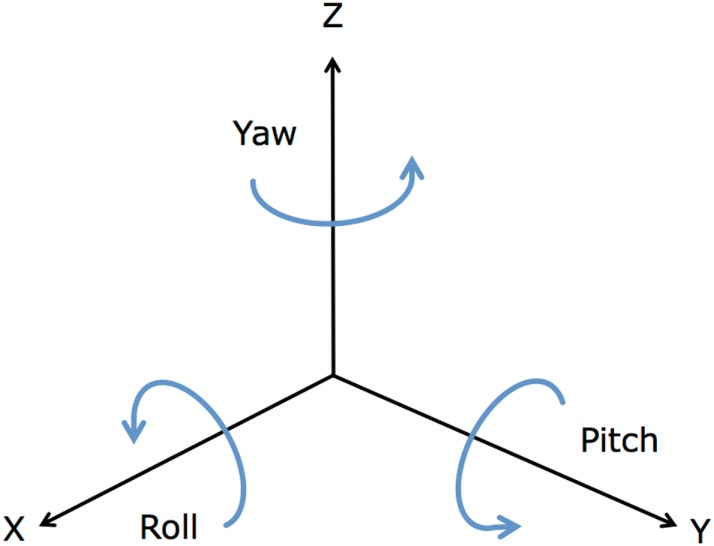
\includegraphics[scale=2]{img/roll_yaw_pitch}
    \caption{A Microsoft által használt fogalmak a fej elfordulására \cite{roll_yaw_pitch}}
\end{figure}

A Microsoft Face API-ja minden fontos tulajdonságot biztosít számunkra, már csak azt kell megnézni, milyen minőségűek ezek a válaszok, mennyire megbízható ez a szolgáltatás. Vizsgáljuk meg a Google Cloud Vision-nél használt képekkel a feldolgozás minőségét különböző minőségű képek esetén  (7.ábra, 8.ábra).

\begin{figure}[h]
 \begin{minipage}{.5\textwidth} 
\centering
    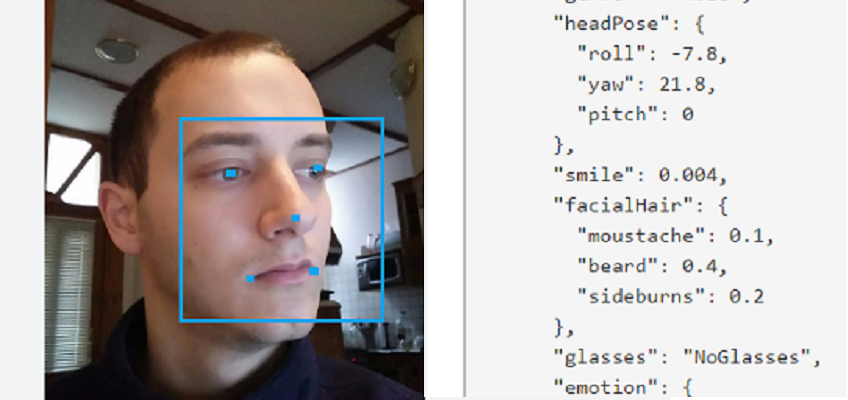
\includegraphics[scale=0.3]{img/mpo_left}
    \caption{Balra néző kép, 21.8 fokos \newline becsült elfordulás}
 \end{minipage}
 \begin{minipage}{.5\textwidth} 
\centering
     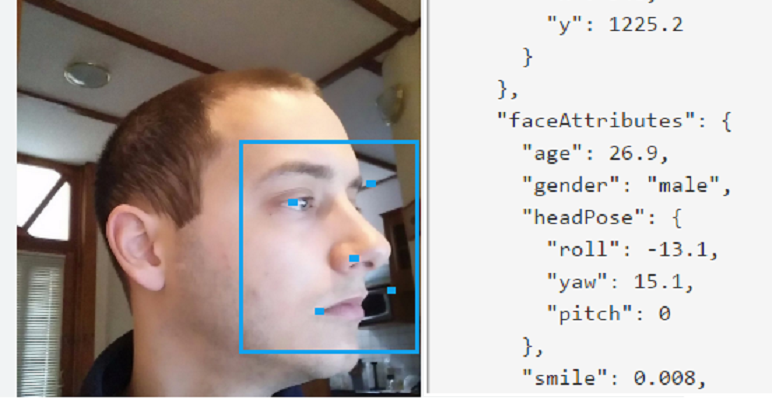
\includegraphics[scale=0.3]{img/mpo_very_left}
     \caption{Balra néző kép, 15 fokos becsült elfordulás}
 \end{minipage}
\end{figure}

Vizsgáljuk meg külön mi történik a feldolgozás eredményével a komolyabb minőségromlás esetén. A feltöltendő képeket az eredeti ~500kb-ról ~40kb-ra csökkentettem, a minőségromlás szemmel látható. Hasonlítsuk össze az erre a két képre adott eredményt (9.ábra, 10.ábra).
\begin{figure}[h]
 \begin{minipage}{.5\textwidth} 
\centering
    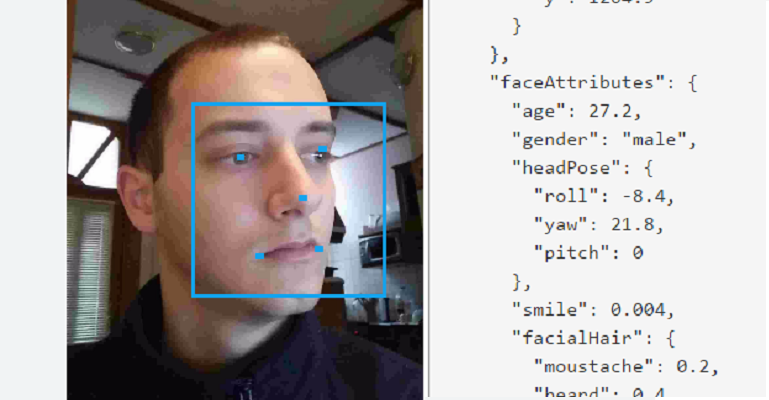
\includegraphics[scale=0.3]{img/mpo_left_compressed}
    \caption{Balra néző tömörített kép, 21.8 fokos becsült elfordulás}
 \end{minipage}
 \begin{minipage}{.5\textwidth} 
\centering
     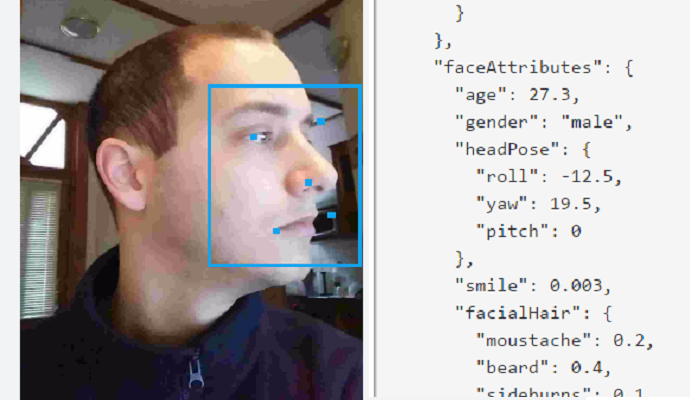
\includegraphics[scale=0.3]{img/mpo_very_left_compressed}
     \caption{Balra néző tömörített kép, 19.5 fokos becsült elfordulás}
 \end{minipage}
\end{figure}

Jól látható, hogy ez az API nem képes olyan széles elfordulás-tartományban dolgozni, mint a már vizsgált Google Cloud Vision. Amennyiben mindkét szem nem látszódik, az orr illesztése rossz helyre kerül és láthatóan az alapján próbálja a másik szemet illeszteni, ami teljesen hibás elfordulás eredményeket ad. Amennyiben kisebb elfordulás elegendő a kihívás-válasz implementációjához, úgy amíg a keresett elfordulás még bőven a megbízhatóan felismert elfordulás tartományon belül van, nem fog problémát okozni a nagy elfordulás esetén mutatott pontatlanság. Mivel ennek a szolgáltatásnak létezik arcösszehasonlító megoldása, mindenképp érdemes azt is megvizsgálni, így mindkét modul azonos szolgáltatáshoz tartozna.

\begin{figure}[h]
 \begin{minipage}{.5\textwidth} 
\centering
    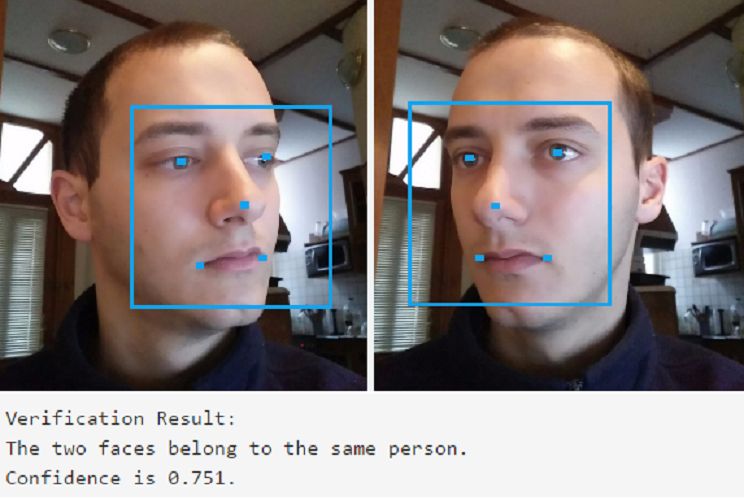
\includegraphics[scale=0.3]{img/mpo_compare}
    \caption{Közepes mértékű elfordulás}
 \end{minipage}
 \begin{minipage}{.5\textwidth} 
\centering
     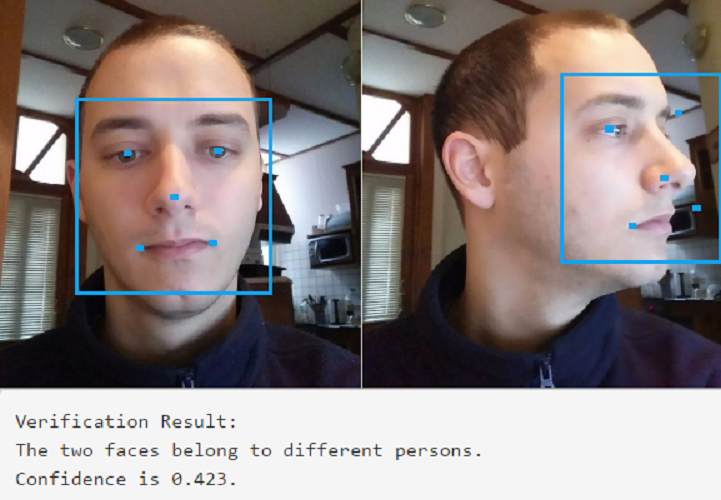
\includegraphics[scale=0.3]{img/mpo_compare_failed}
     \caption{Nagy mértékű elfordulás esetén nem megbízható}
 \end{minipage}
\end{figure}

Jól látható, hogy az elfordulás mértéke drasztikusan befolyásolja az összehasonlítás megbízhatóságát. Ez még nem feltétlen probléma. A kihívás-válasz lefutása alapján nagy valószínűséggel lesz olyan képkockánk is, amikor a felhasználó a kamerába néz, így érdemes lenne nem csak maximum elfordulást keresni, hanem egy minimumot is egy bizonyos küszöbszám alatt. Ennek segítségével tudnánk mindenképpen olyan képet küldeni összehasonlításra az igazolványképpel, ami kamerába néz, megkönnyítve a képfeldolgozó szolgáltatás dolgát.
A Microsoft Face API-t megvizsgálva megállapítható, hogy minden számunkra szükséges funkcióval rendelkezik, azokat kellő körültekintéssel használva megbízható eredményeket kapunk. Ezért ezt érdemes beépíteni a szakdolgozat keretein belül.

\subsubsection{Face++}
Utolsó online megoldásként a Face++ szolgáltatását vizsgáltuk meg, amit többek között a Lenovo is használ saját célra. Mindenképpen pozitívum, hogy nincsen használati limit az ingyenes csomagban sem, viszont nem enged párhuzamos képfeldolgozást. 83 különböző tulajdonságot ad vissza egy felismert arcról, többek között a számunkra fontos "yaw\_angle"-t is \cite{FACEPP}. Ezen kívül a szokásos életkor, nem, különböző testrészek pozícióját az arcon és még sok egyebet ismer fel.
\\Összehasonlításra szintén használható, a Microsofthoz hasonló módon két képet vár (vagy egy előre felismert képnek az azonosítóját), amire három különböző százalékos értéket kapunk vissza \cite{FACEPP_COMPARE}. Ezek a százalékos értékek különböző hibaszázalék mellett mutatják annak a valószínűségét, hogy a két kép ugyanahhoz a fizikai személyhez tartozik. Ez különösen akkor lehet hasznos, ha különböző érzékenységű adatokat akarunk védeni a szoftverünkkel, és így magas érzékenységű adathoz alacsonyabb hibahatárt várunk. Egy negyedik százalékos érték maga a végleges valószínűség, nekünk egyelőre elég lesz azzal foglalkozni. Érdemes lehet főleg a limitmentessége és mindkét használható modulja miatt beépíteni a szakdolgozat keretében ezt a szolgáltatást is. 

\subsubsection{Egyéb vizsgált lehetőségek}

\begin{itemize}
\item mesterséges intelligencia függvénytárak (Dlib, opencv) offline saját megoldásra jó opciónak tűnnek, ám ezek megismerése és használata hosszabb időt igényel, minthogy beleférjen a szakdolgozat kereteibe. Bemutató videók alapján akár szemmozgás, pislogás felismerésére is használható, hosszútávon mindenképpen megfontolandó ennek használata/beépítése.
\item BioID regisztrációhoz kötött, de ingyenes. Minimum két kép feltöltésével jelenlét ellenőrzést kínál hangsúlyozva, hogy jelenleg könnyen kijátszható a rendszer. Kihívás - válasz kritérium csatolható a kéréshez, ilyenkor ennek is meg kell felelni (arcelfordítás, akár egymás után többször is). Ez a működés szerinti csoportosításnak az a fele, amelyik saját maga implementálja a kihívást.
\item Lambda Labs Face Recognition API egyik számunkra szükséges modulhoz sem nyújt segítséget.
\item FaceR szintén nem nyújt segítséget számunkra.
\end{itemize}

\subsection{Választott megoldások}
Összegezve a különböző szolgáltatásokról gyűjtött adatokat a következő összefoglalást készíthetjük:
\begin{center}
	\begin{tabular}{|p{3cm}|p{2cm} |p{2cm} | p{3cm}|p{3cm}|}
   	\hline
	\textbf{Szolgáltatás neve} & \textbf{Online / Offline} & \textbf{Szükséges modulok megléte} & \textbf{Képfeldolgozás minősége} &\textbf{ Összehasonlítás minősége} \\ \hline
	Google Cloud Vision & Online & Arc elfordulás & Széles skálán érzékeli az elfordulást tömörítés esetén is & Nincsen \\ \hline
	IBM Watson & Online & Egyik se & Nincsen & Nincsen \\ \hline
	Microsoft Project Oxford & Online & Mindkettő & Közepes mértékű elfordulásig tömörítés esetén is megfelelő & Közepes mértékű elfordulásig tömörítés esetén is megfelelő\\ \hline
	Face++ & Online & Mindkettő & Tesztelni kell, nincsen online felülete & Tesztelni kell, nincsen online felülete \\ \hline
	Google Mobile Vision & Offline (csak iOS és Android) & Arc elfordulás & Tesztelni kell, nincsen online felülete & Nincsen \\ \hline
	\end{tabular}
\end{center}

Ezek alapján a Microsoft Project Oxford és a Face++ beépítése illetve tesztelése mellett döntöttünk a szakdolgozat keretein belül.

\newpage